\newpage

\section{Partial Redundancy Elimination}
Partial redundancy elimination (PRE) is a global optimization introduced by Morel and Renvoise\cite{morel1979global}. It
combines and extends two other techniques: common subexpression elimination and loop-invariant code motion. 

An expression is partially redundant at point p if it
is redundant along some, but not all, paths that reach
p. PRE converts partially-redundant expressions into
redundant expressions. The basic idea is simple. First,
it uses data-flow analysis to discover where expressions
are partially redundant. Next, it solves a data-flow
problem that shows where inserting copies of a computation would convert a partial redundancy into a full
redundancy. Finally, it inserts the appropriate code and
deletes the redundant copy of the expression.

A key feature of PRE is that it never lengthens an
execution path. To see this more clearly, consider the
example shown in Figure \ref{fig:p82}. In the fragment on the left, the second
computation of \texttt{x + y} is partially redundant; it is only
available along one path from the if. Inserting an evaluation of 
\texttt{x + y} on the other path makes the computation
redundant and allows it to be eliminated, as shown in
the right-hand fragment. Note that the left path stays
the same length while the right path has been shortened.


\begin{figure}[H]
    \centering
     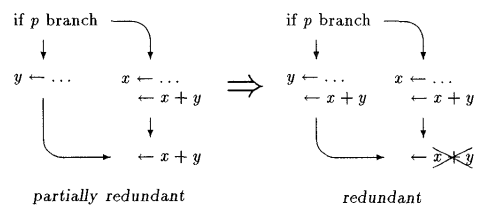
\includegraphics[width=0.5\textwidth]{p82.png}
         \caption{}
         \label{fig:p82}
\end{figure}


Loop-invariant expressions are also partially redundant,
as shown in Figure \ref{fig:p83}. On the left, \texttt{x + y} is
partially redundant since it is available from one predecessor 
(along the back edge of the loop), but not the
other. Inserting an evaluation of \texttt{x + y} before the loop
allows it to be eliminated from the loop body.


\begin{figure}[H]
    \centering
     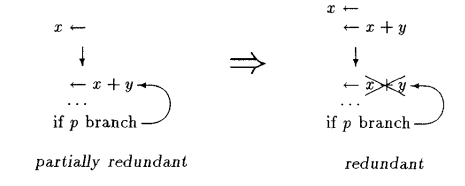
\includegraphics[width=0.5\textwidth]{p83.png}
         \caption{}
         \label{fig:p83}
\end{figure}


\subsection{Finding Partially Available Expressions}

For every expression, we can do a dataflow analysis.

\begin{center}
    \begin{tabular}{|c|c|}
   \hline Direction & Forward\\
   \hline Meet operator & \( \cup \)\\
   \hline Lattice & \( \{ 0,1 \} \)\\
   \hline Top(T) & \( 0 \)\\
   \hline Bottom &  \( 1 \)\\
   \hline Boundary condition for entry node & \( 0 \) \\  
   \hline Initialization for internal nodes & \(\mathrm{T}\) \\
   \hline Finited escending chain? &\checkmark  \\
   \hline Transferfunction  &  \( PAVOUT[i] =  (PAVIN[i] - KILL[i]) \cup AVLOC[i]\)\\
   \hline Monotone\&Distributive?  & \checkmark \\
   \hline AVLOC  & {Expression is {\color{blue}locally available (AVLOC)} if downwards exposed.  }\\
   \hline KILL & Expression is {\color{blue}killed ( KILL)} if any assignments to operands. \\
   \hline
   \end{tabular}  
   \end{center}


   \begin{figure}[H]
    \centering
     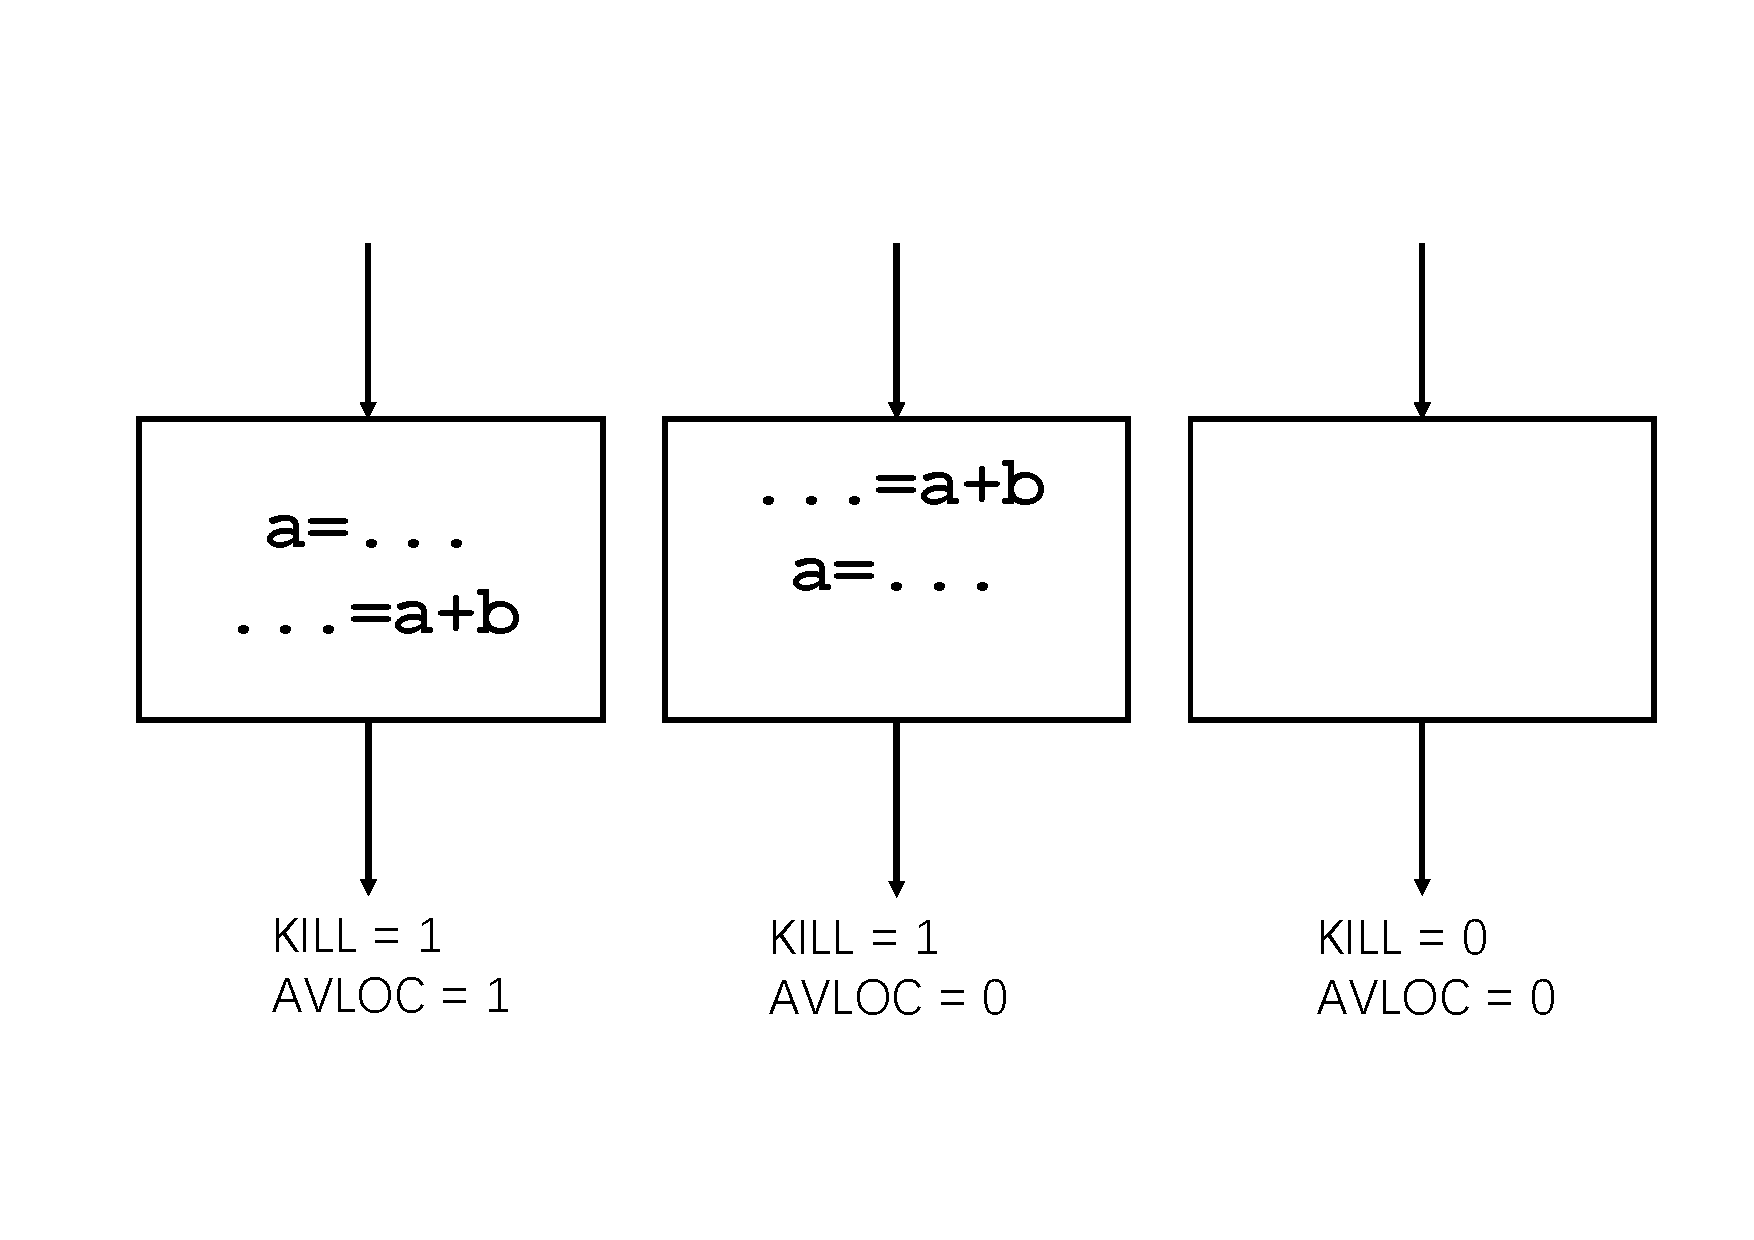
\includegraphics[width=0.8\textwidth]{p84.pdf}
         \caption{For \texttt{a+b}, the result of  Partially Available Expressions's transfer function within a basic block.}
         \label{fig:p84}
\end{figure}



\begin{figure}[H]
    \centering
     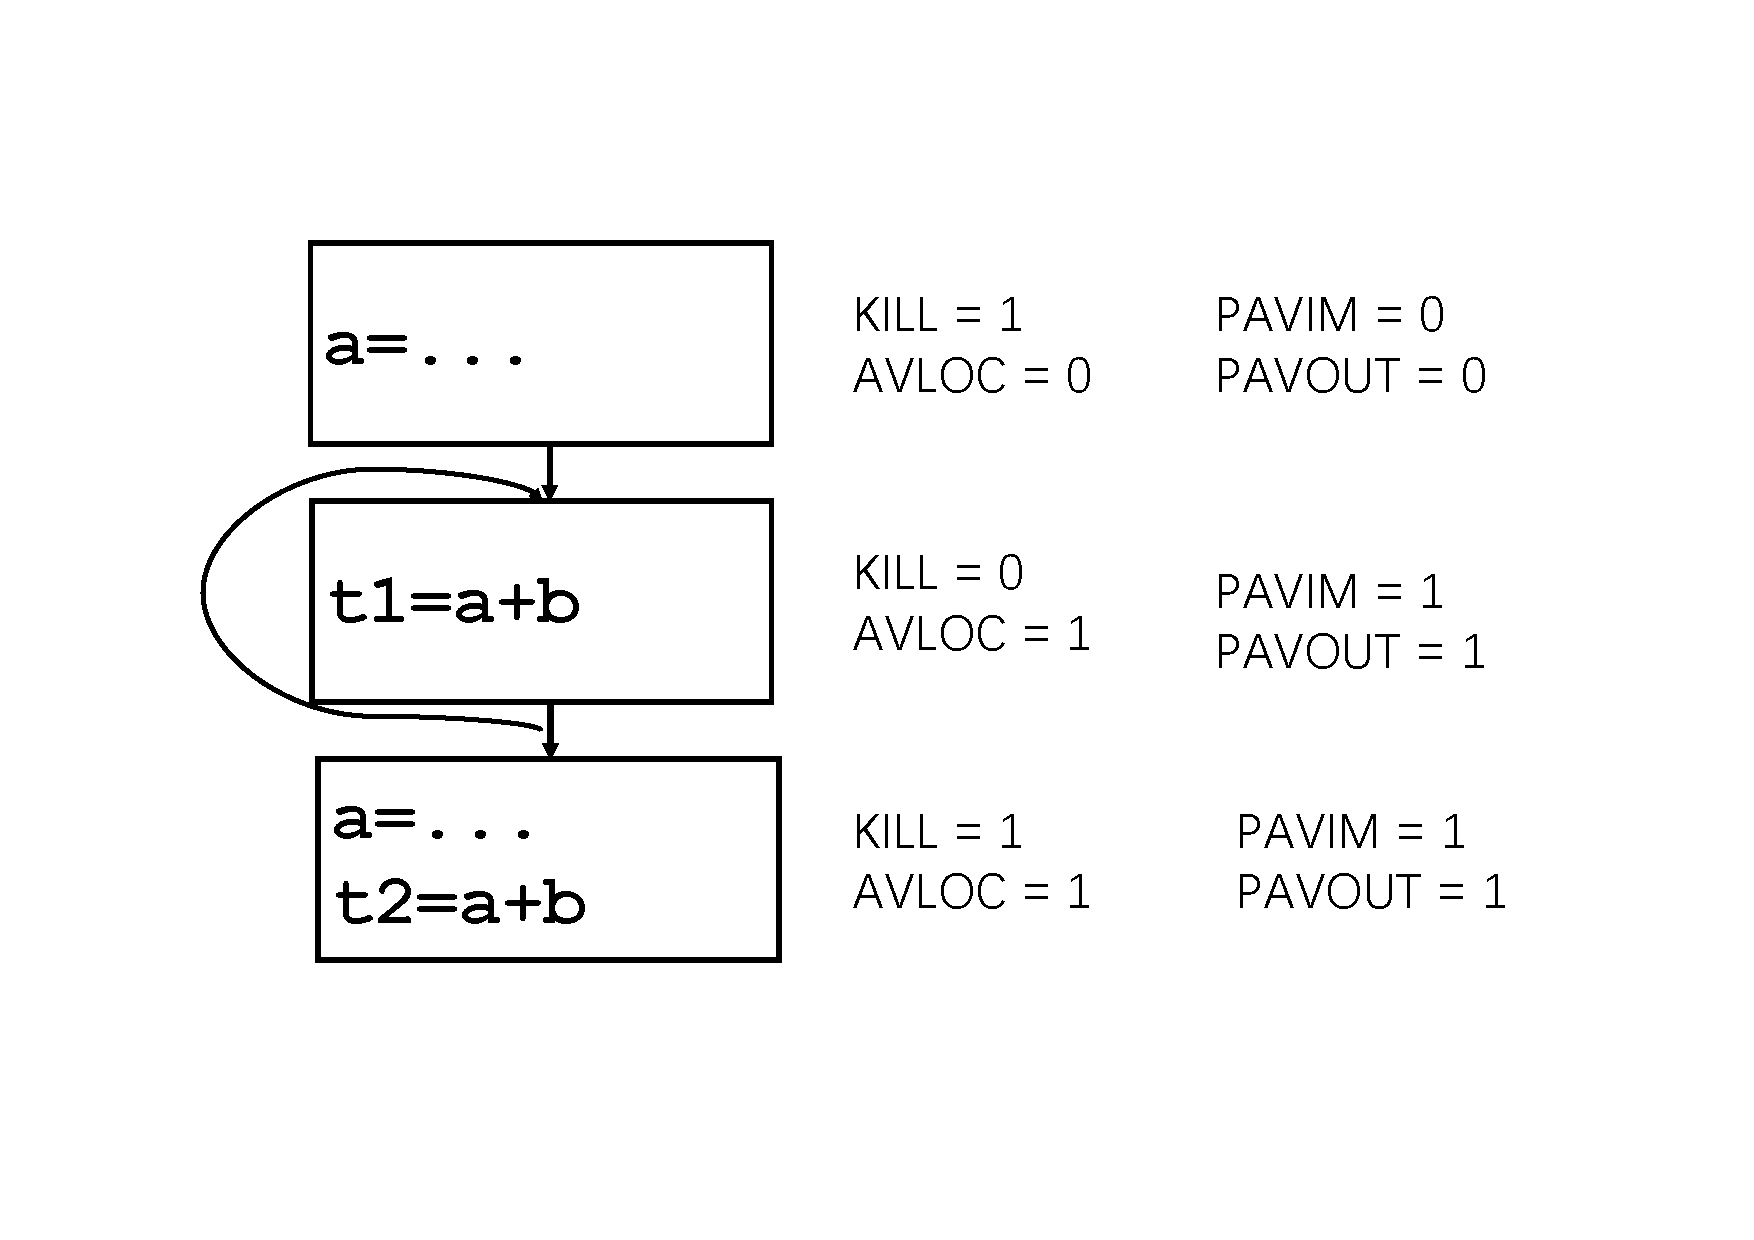
\includegraphics[width=0.8\textwidth]{p85.pdf}
         \caption{For \texttt{a+b}, the result Partially Available Expressions of dataflow analysis.}
         \label{fig:p85}
\end{figure}

\subsection{Finding Anticipated Expression}

For PRE, care must be taken that the hoisting would do no harm: Never introduce
 a new expression along any path. Otherwise the
hoisting will lengthen at least one trace of the program, defying optimality; even
worse, if the hoisted instruction throws an exception, the program’s semantics
change.



\begin{definition}{Local Anticipability(ANTLOC)}
An expression may
be locally anticipated in a block i if there is at least one
computation of the expression in the block i, and if the
commands appearing in the block before the first computation 
of the expression do not modify its operands. 
\end{definition}


\begin{center}
    \begin{tabular}{|c|c|}
   \hline Direction & backward\\
   \hline Meet operator & \( \cap \)\\
   \hline Lattice & \( \{ 0,1 \} \)\\
   \hline Top(T) & \( 1 \)\\
   \hline Boundary condition for exit node & \( 0 \) \\  
   \hline Initialization for internal nodes & \(\mathrm{T}\) \\
   \hline Finited escending chain? &\checkmark  \\
   \hline Transferfunction  &  \( ANTIN[i] = ANTLOC[i] \cup (ANTOUT[i] - KILL[i])\)\\
   \hline Monotone\&Distributive?  & \checkmark \\
   \hline ANTLOC & Expression is locally {\color{blue}anticipated(ANTLOC))} is upward exposed.\\
   \hline
   \end{tabular}  
   \end{center}

   \begin{figure}[H]
    \centering
     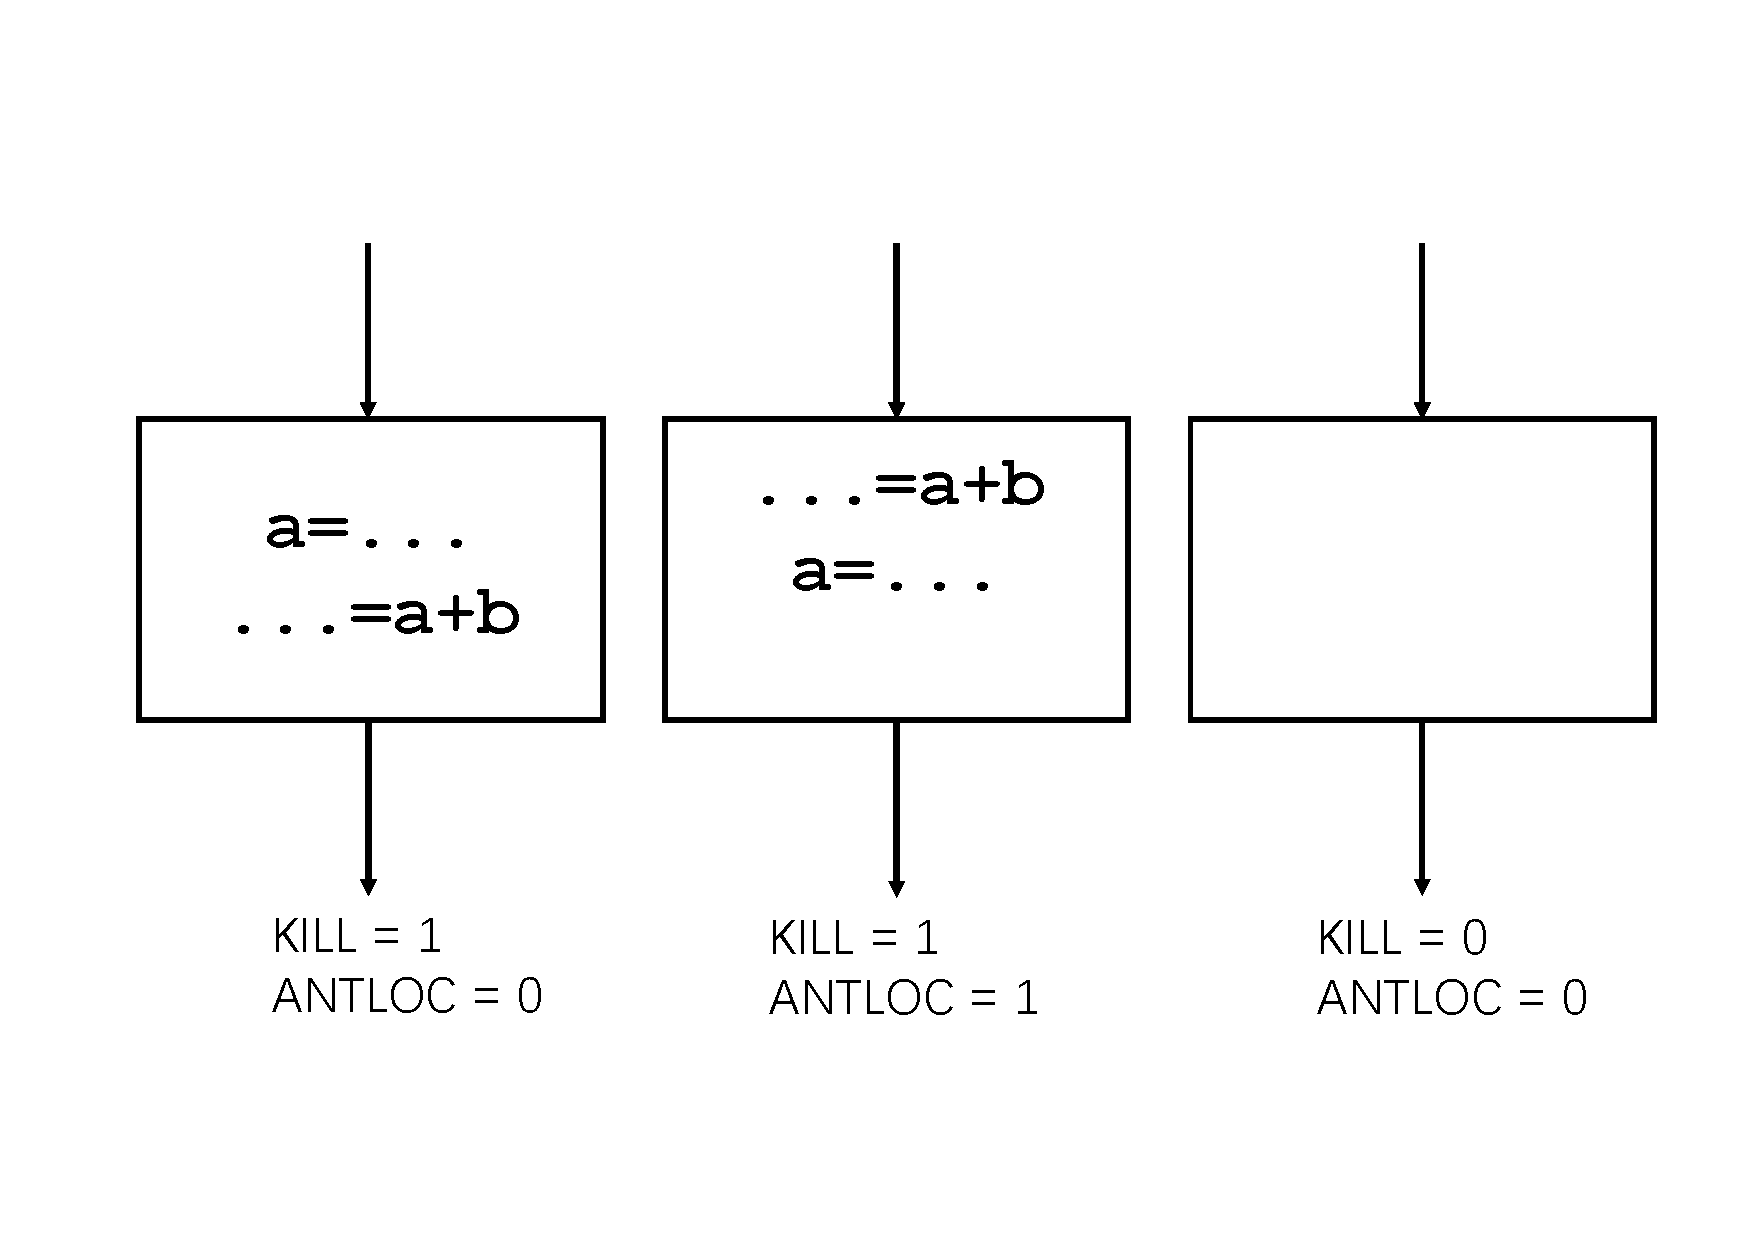
\includegraphics[width=0.8\textwidth]{p86.pdf}
         \caption{For \texttt{a+b}, the result of Anticipated Expression's transfer function within a basic block.}
         \label{fig:p86}
\end{figure}



\begin{figure}[H]
    \centering
     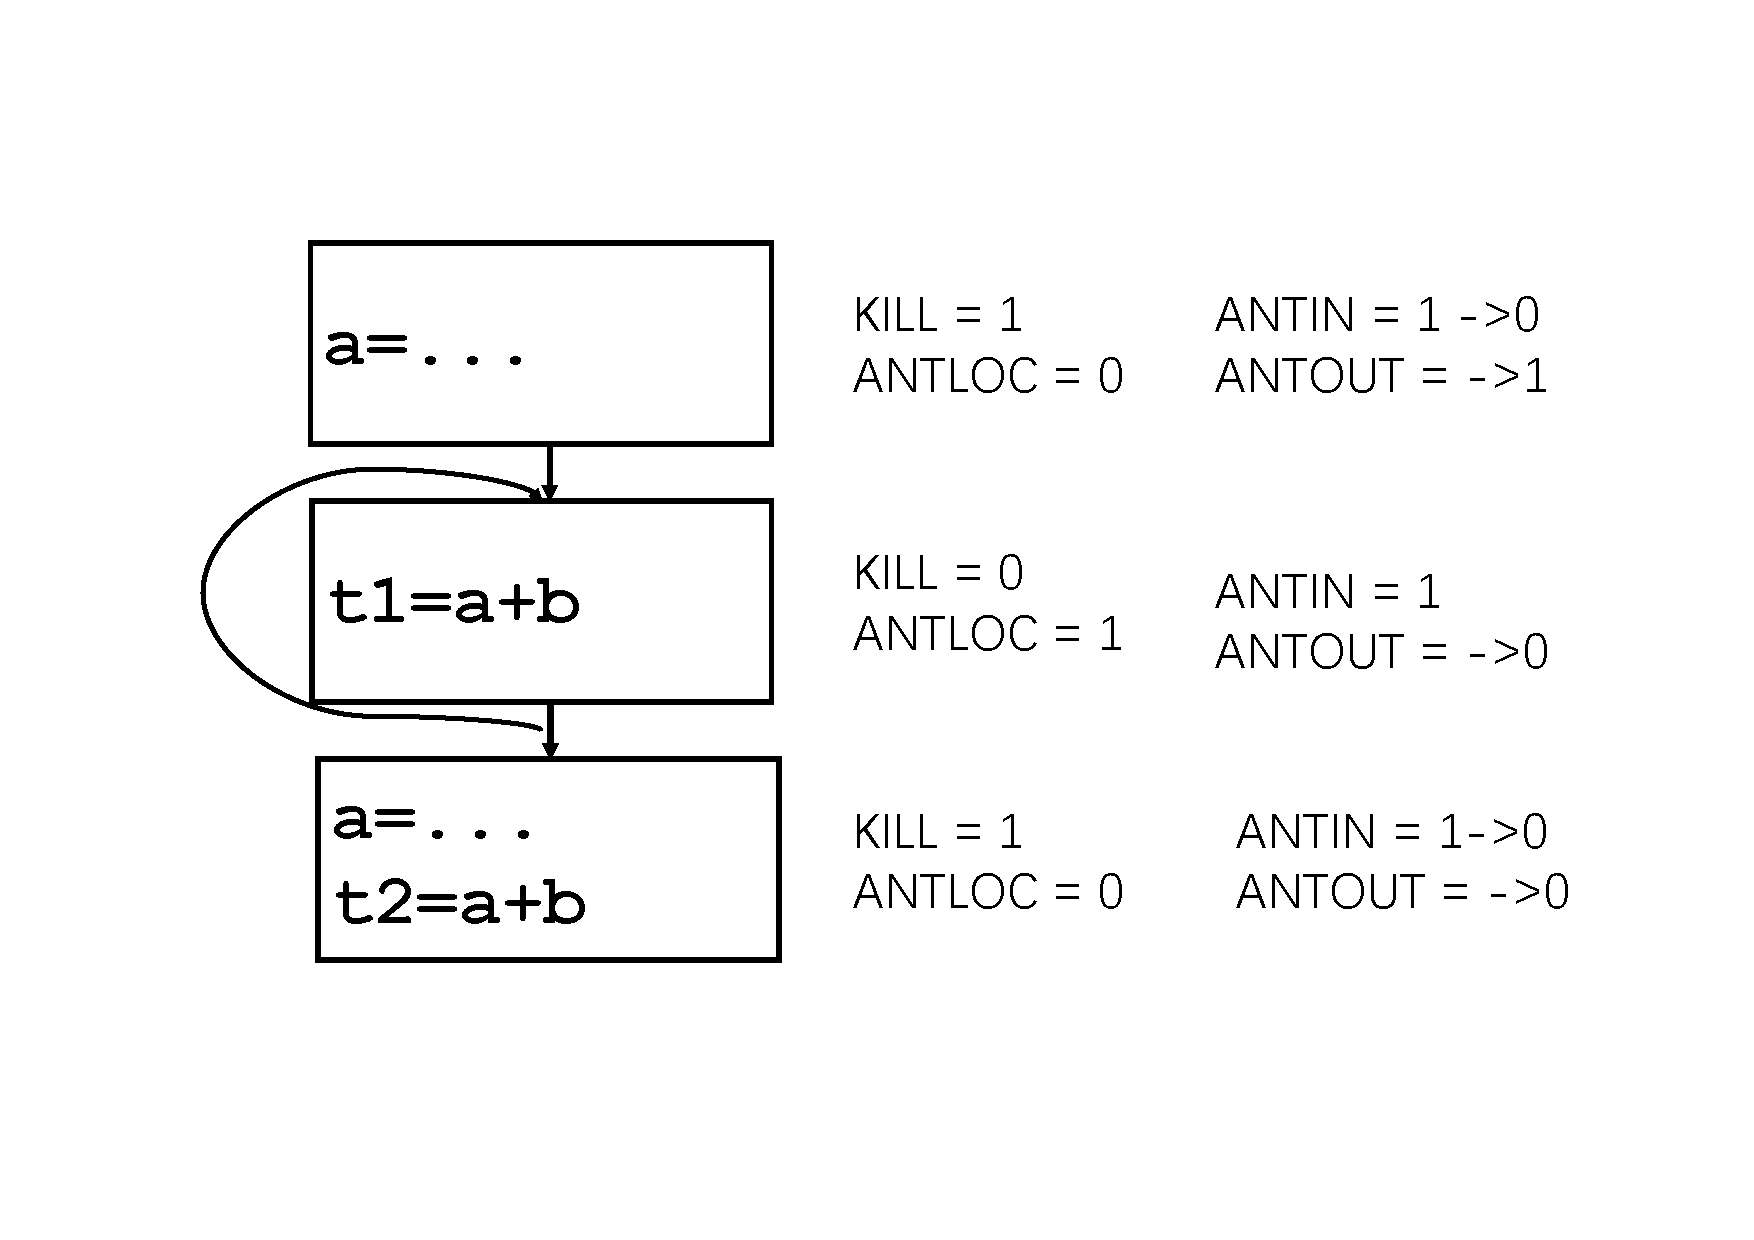
\includegraphics[width=0.8\textwidth]{p87.pdf}
         \caption{For \texttt{a+b}, the result Anticipated Expression of dataflow analysis.}
         \label{fig:p87}
\end{figure}


\subsection{Where Do we Want to Insert Computations?}


\begin{figure}[H]
    \centering
     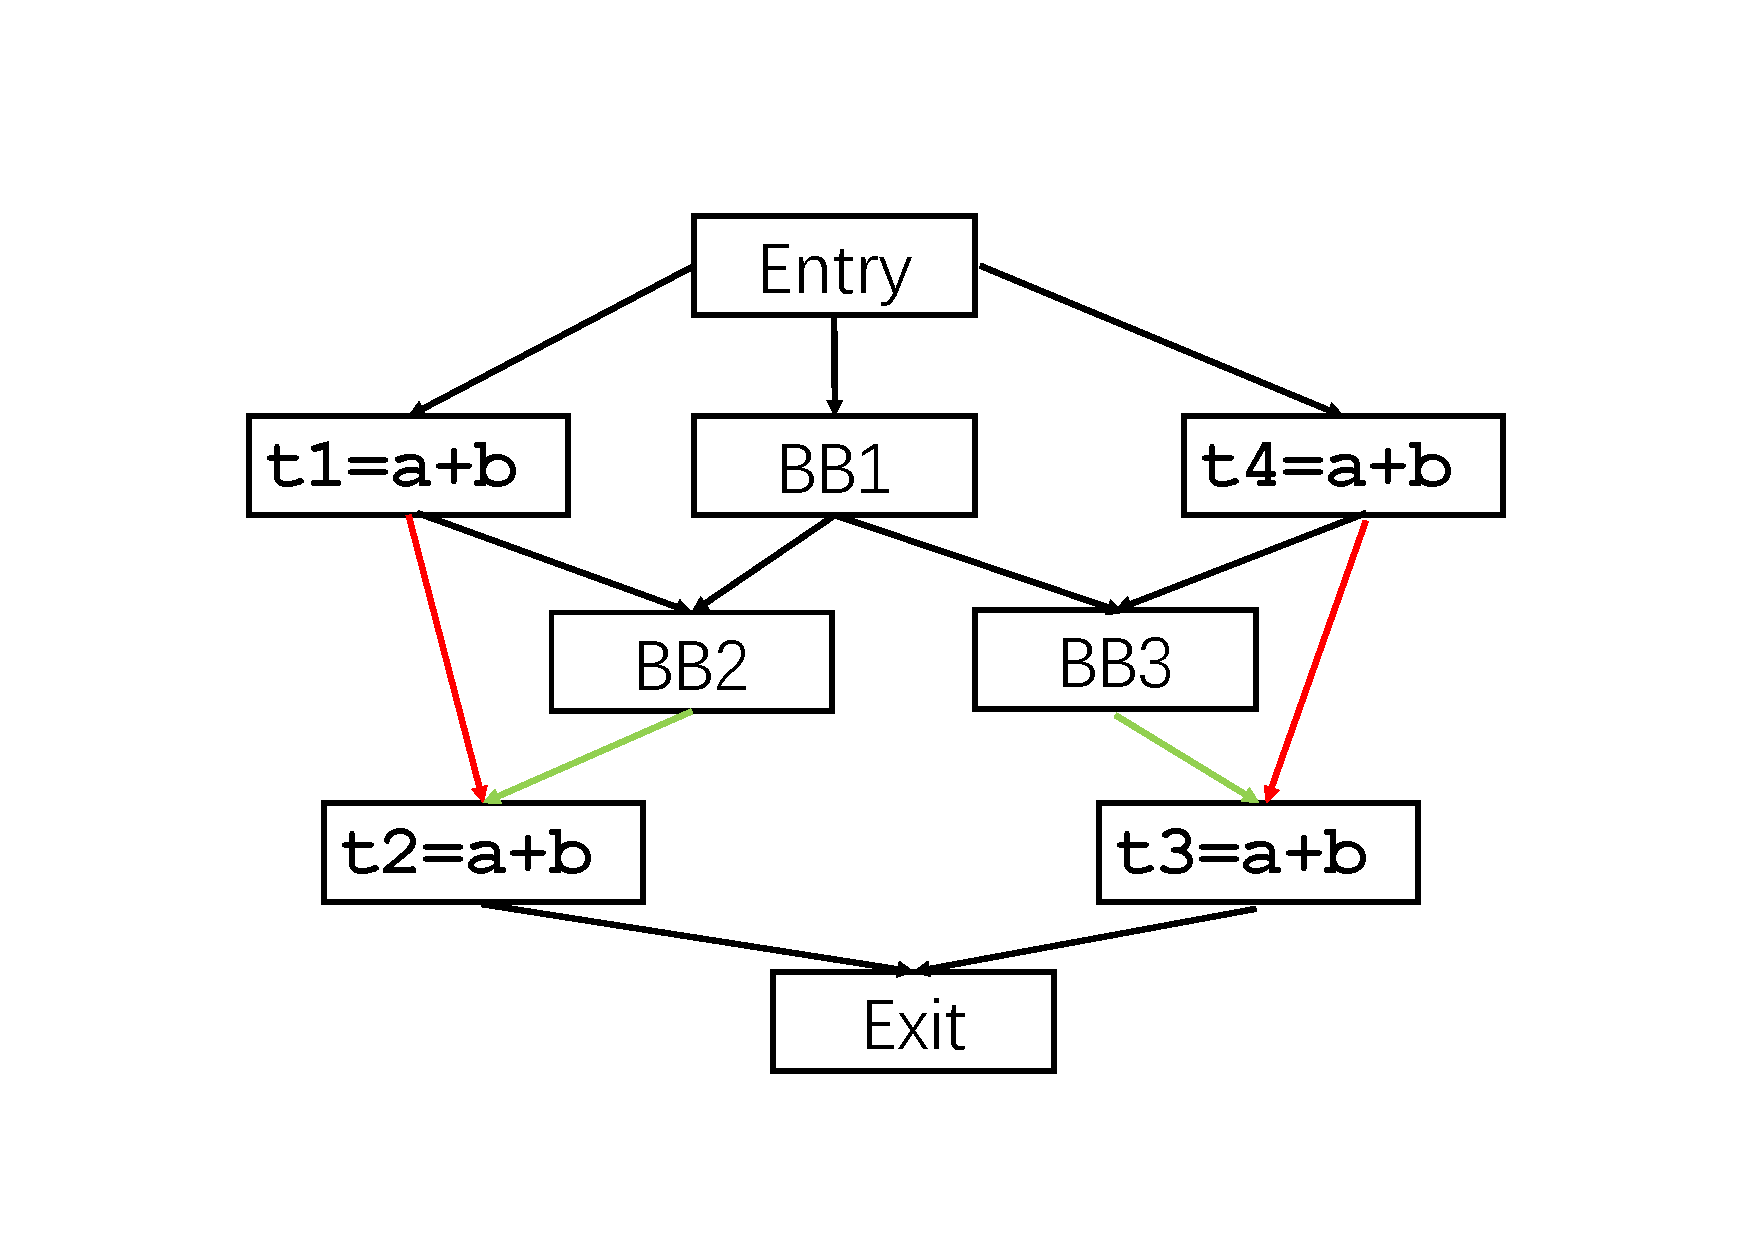
\includegraphics[width=0.8\textwidth]{p88.pdf}
         \caption{For \texttt{a+b}, \texttt{t2 = a + b} and \texttt{t3 = a + 4} are both partially redundant. But where can we insert the new computation \texttt{a + b} in order to optimally eliminate redundancy?
         The best choice is BB1 because this wil  make \texttt{a + b} fully redundant. But if we insert to BB2 and BB3, there are some path that calculate \texttt{a + b} more than once (e.g. Entry$\rightarrow$\texttt{t1= a+b} $\rightarrow$ BB2$\rightarrow$\texttt{t2= a+b}) }
         \label{fig:p88}
\end{figure}

We define "\textbf{Placement Possible }"(PP) dataflow analysis. First of all, we are only going to place computations at the end of the blocks. 
We want to insert the computation at the earliest place where our \textbf{Placement Possible }is true. If the \textbf{Placement Possible }is true output of a block(PPOUT), it means 
it is fine to insert at the end of this block or earlier. If it is true athe the beginning of the block, it means we could insert it at the beginning of the block or earlier. Becuase we want to
insert it at the end of the block, so if \textbf{Placement Possible }is true at the beginning of the block(PPIN), you won't insert it in the block, it means you need to take care of something before.
So when PPIN is true, it really means is for every predecessor block, it is either possible to keep moving it back and make it fully redundant by placing in that block or earlier or it is not necessary because 
it is already generatedin one of those blocks. 

We insert if PPOUT is true and either PPIN is false so we cannot move it back any further or if we locally kill it then clearly we have to insert it here because trying to insert it earlier would not work. And we only want to insert it if it is not 
already available.


We want to delete an expression where PPIN is true (somehow we make it fully redundant) and it is anticipated locally.


For safety reasons, if we want to place at output of a block, we want to place at entry of all successors. (PPOUT)

$$
\text { PPOUT[i] }=\left\{\begin{array}{cl}
0 & i=\text { entry } \\
\bigcap_{s \in \operatorname{succ}(i)} \operatorname{PPIN}[\mathrm{s}] & \text { otherwise }
\end{array}\right.
$$


When PPIN is true, if means 
\begin{itemize}
\item we have a local computation to place, or a placement at the end of this block which we can move up 
\item  we want to move computation to output of all predecessors where expression is not already available (don’t insert at input) (for every predecessor,)
\item we gain something by moving it up (PAVIN heuristic) (not too far)
\end{itemize}

$$
\operatorname{PPIN}[\mathrm{i}]=\left\{\begin{array}{cc}
0 & i=\text { exit } \\
([\text { ANTLOC[i] } \cup \text { (PPOUT }[i]-\operatorname{KILL}[i])] & \\
\cap \bigcap_{p \in \text { preds }(i)}(\text { PPOUT }[p] \cup \text { AVOUT }[p]) & \text { otherwise } \\
\cap \text { PAVIN }[i]) &
\end{array}\right.
$$




\begin{figure}[H]
    \centering
     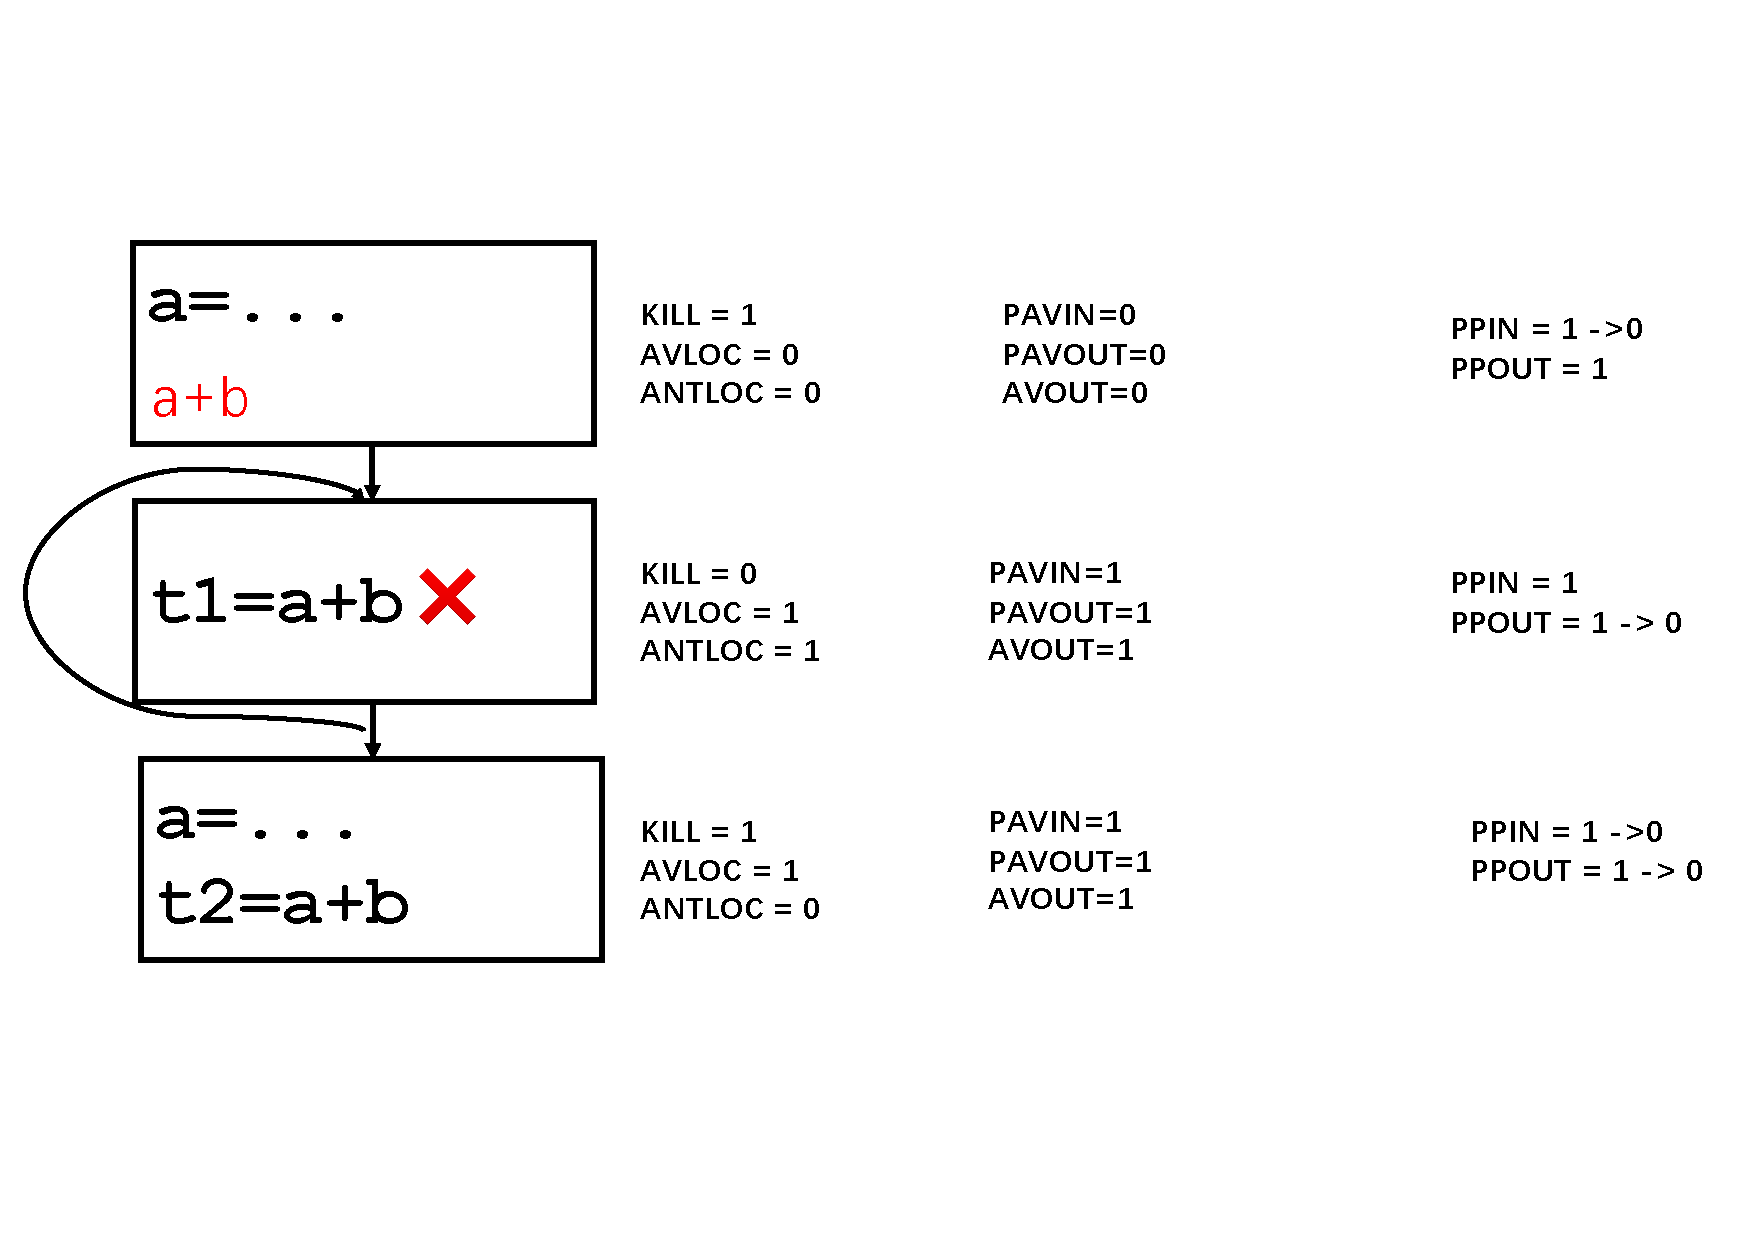
\includegraphics[width=0.8\textwidth]{p102.pdf}
         \caption{Example for PRE for \texttt{a+b}}
         \label{fig:p102}
\end{figure}

\begin{figure}[H]
    \centering
     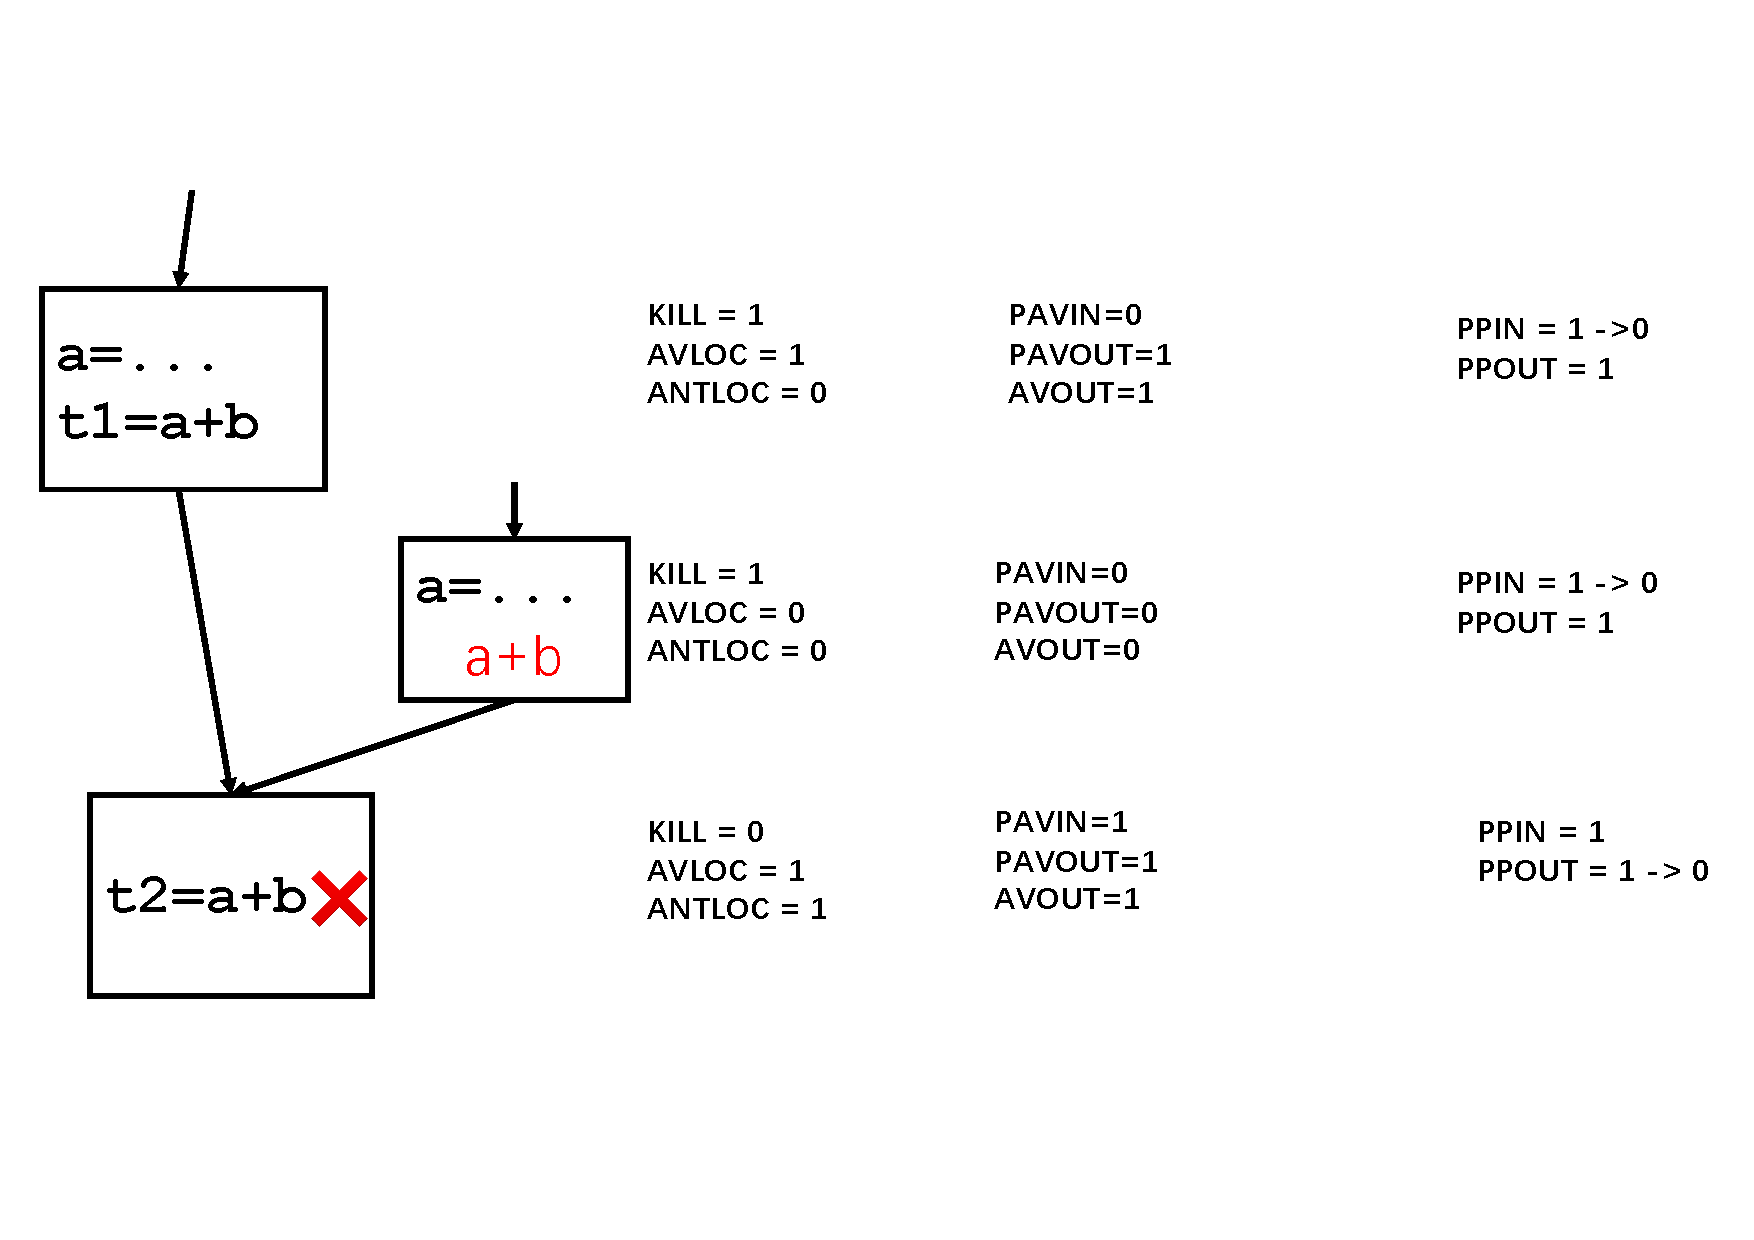
\includegraphics[width=0.8\textwidth]{p103.pdf}
         \caption{Example for PRE for \texttt{a+b}}
         \label{fig:p103}
\end{figure}
\subsubsection{Safety}

It is  safe to insert only if anticipated. 

$$
\text { PPIN[i] } \subseteq(\text { PPOUT[i] - KILL[i]) U {\color{red}ANTLOC}[i] }
$$


$$
\text { PPOUT[i] }=\left\{\begin{array}{cl}
0 & i=\text { entry } \\
\bigcap_{s \in \operatorname{succ}(i)} \operatorname{PPIN}[\mathrm{s}] & \text { otherwise }
\end{array}\right.
$$

$$
{\color{red}\text{INSERT}} \subseteq \text{PPOUT} \subseteq {\color{red}\text{ANTOUT}}
$$

So it is safe.

\subsection{Perform}
On every path from an INSERT, there is a DELETE.


\subsection{Limiations}




\subsection{A new way to think about partial redundancy}


























We want to insert the new computation where it is not partially available there.


\begin{definition}{Anticipable(Very Busy) Expression}
    An	expression	e	is	anticipable	at	a	program	point	p	
    if	e will	be	computed	along	every	path	from	
    p	to	p$_{\mathrm{end}}$,	and	no	 variable	in	e	is	
    redefined	until	its	computation. It	is	safe	to	move	
    an	expression	to	a	basic	block	where	
    that	expression	is	anticipable. By	"safe"	we	mean	
    "performance	safe",	i.e.,	no	extra computation	
    will	be	performed.	Notice	that	if	an	expression	
    e	is	computed	at	a	basic block	where	it	is	both     available
    and	anticipable,	then	that	
    computation	is	clearly	redundant.		

    \begin{figure}[H]
        \centering
         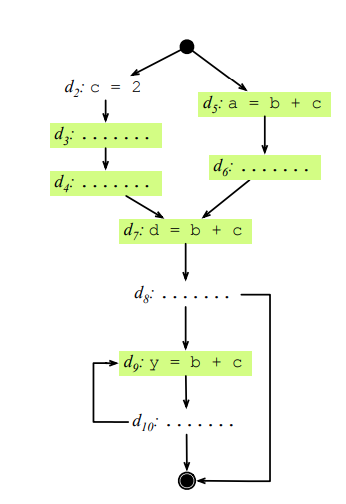
\includegraphics[width=0.5\textwidth]{p89.png}
             \caption{For \texttt{b+c}, the {\color{green}green} blocks are anticipable points. }
             \label{fig:p89}
    \end{figure}
\end{definition}



The key to partial redundancy
elimination is deciding where to add
computations of an expression to
change partial redundancies into full
redundancies (which may then be
optimized away). There	are	now	two	steps	that	we	must	
perform:

\begin{itemize}
\item First,	we	find	the	earliest	places	in	which	
we	can	move	the	computation	of	an	
expression	without	adding	unnecessary	
computations	to	the	CFG.	This	step	is	like	
pushing	the	computation	of	the	
expressions	up.	
\item Second,	we	try	to	move	these	
computations	down,	closer	to	the	places	
where	they	are	necessary,	without	adding	
redundancies	to	the	CFG.	This	phase	is	like	
pulling	these	computations	down	the	CFG. So	that	we	can,	
for	instance,	reduce	register	
pressure.
\end{itemize}

\begin{figure}[H]
    \centering
     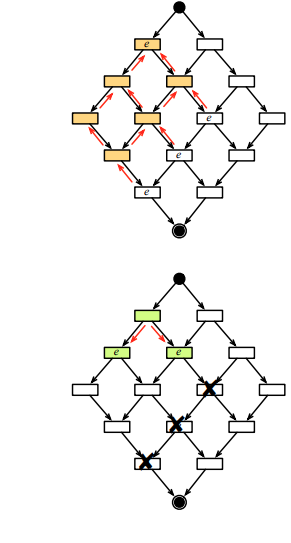
\includegraphics[width=0.3\textwidth]{p90.png}
         \caption{Pushing up, Pulling down.}
         \label{fig:p90}
\end{figure}

\subsubsection{Earliest	Placemen}

We	must	now	find	the	earliest	possible	places	where	we	
can	compute	the	target	expressions.	Earliest	in	the	sense	that	p1	comes	before	p2	if	p1	precedes	
p2	in	any	topological	ordering	of	the	CFG.

\begin{figure}[H]
    \centering
     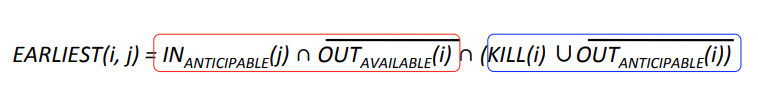
\includegraphics[width=0.6\textwidth]{p91.png}
         
         \label{fig:p91}
\end{figure}


For the {\color{red} Fisrt} part, We	can	move	an	expression	e	to
an	edge	ij	only	if	e	is	anticipabled	at	the	entrance
of	j.	 If	the	expression	is	available	at	the	beginning	of	the	edge,
then	we	should	not	move	it	there.	
But the {\color{blue} Second} part, If	an	expression	is	anticipable	at	i,	
then	we	should	not	move	it	to	ij,	because	we	can	move	it	to	before	i.	
On	the	other	hand,	if	i	kills	the	expression,	then	it	cannot	
be	computed	before	i.


\begin{figure}[H]
    \centering
     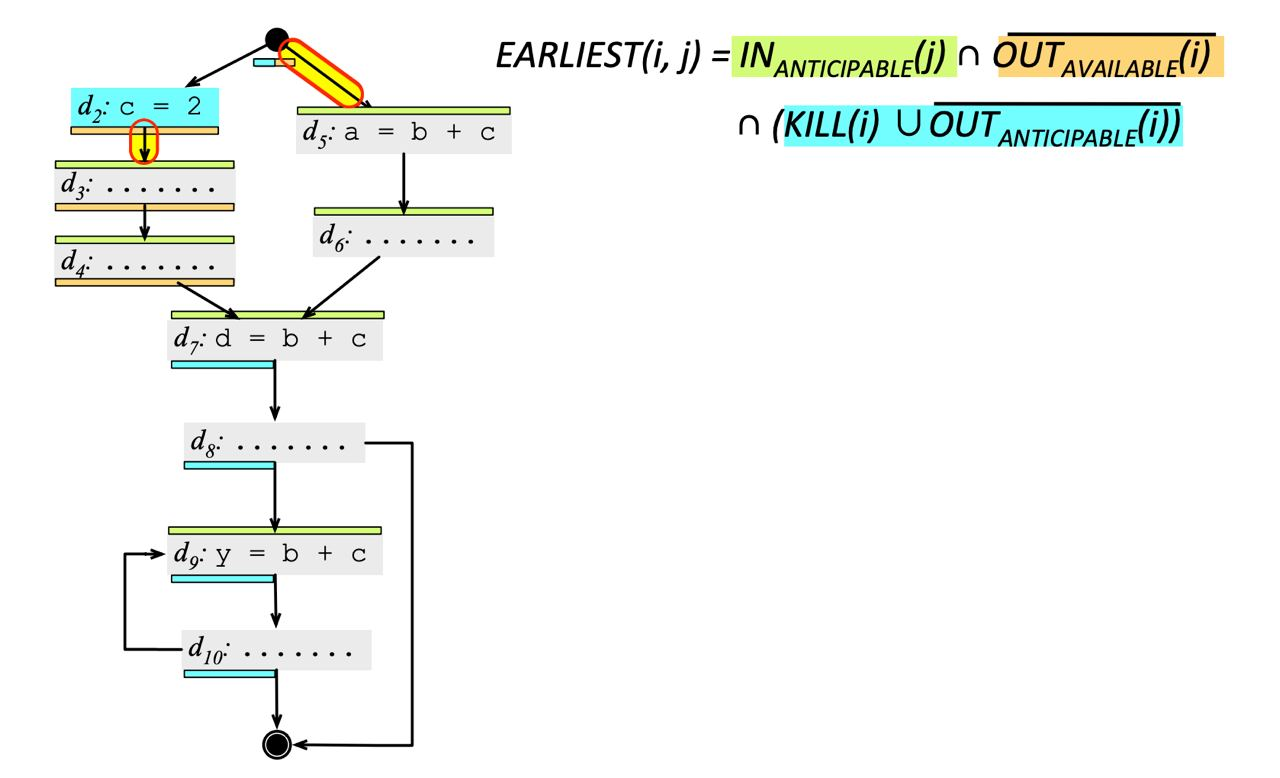
\includegraphics[width=0.8\textwidth]{p92.jpg}
         \caption{An example for calculating EARLIEST.}
         \label{fig:p92}
\end{figure}

\subsubsection{Latest	Placement}


$$
\begin{aligned}
&\operatorname{IN}_{\text {LATER }}(j)=\cap_{i \in \operatorname{pred}(j)} \operatorname{LATER}(i, j) \\
&\operatorname{LATER}(i, j)=\operatorname{EARLIEST}(i, j) \cup\left(\operatorname{IN}_{\text {LATER }}(i) \cap \overline{\operatorname{EXPR}(i)}\right). \\
&
\end{aligned}
$$


LATER(i,j)	is	true	if	we	can	move	the	computation	of	the	
expression	down	the	edge	ij.	 An	expression	e	is	in	
EXPR(i)	if	e	is	computed	at	i.	This	predicate	is	also
 computed	for	edges,	although	we	
have	IN$_\mathrm{LATER}$	being	computed	for	nodes.	



% $$
% \operatorname{LATER}(i, j)=\operatorname{EARLIEST}(i, j) \cup\left(\operatorname{IN}_{\text {LATER }}(i) \cap \overline{\operatorname{EXPR}(i)}\right). 
% $$

For \( \mathrm{LATER}(i,j) \): If	EARLIEST(i,	j)	is	true,	
then	\( \mathrm{LATER}(i,j) \)	is	also	true,	as	we	
can	move	the	computation	of	e	to	edge	ij	without	
causing	redundant	computations. 	If	\( IN_{\mathrm{LATER}}(i,j) \)	is	true,	
and	the	expression	is	not	used	at	i,	
then	LATER(i,j)	is	true.	If	the	expression	is	used	at	i,	then	there	is	no	point	in	
computing	it	at	ij,	because	it	will	be	recomputed	at	i
anyway.	


For \( IN_{\mathrm{LATER}}(i,j) \), it is	a	condition	that	
we	propagate	down.	If	all	the	predecessors	of	a	
node	j	accept	the	
expression	as	nonredundant,	then	we	can	
compute	the	expression	
down	on	j.	

\begin{figure}[H]
    \centering
    \begin{subfigure}{0.3\textwidth}
    \centering
        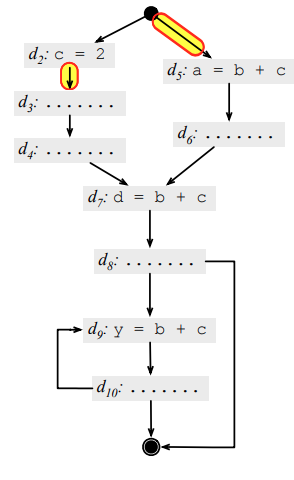
\includegraphics[width=\textwidth]{p94.png}
        \caption{For \texttt{b+c}, 	two	
        earliest	placement	
        points is colored in red.}
        \label{fig:p94}
    \end{subfigure}
    \begin{subfigure}{0.4\textwidth}
    \centering
        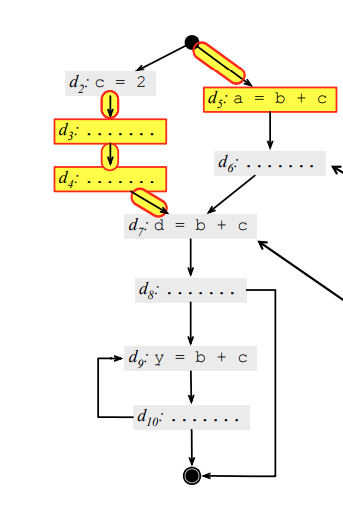
\includegraphics[width=\textwidth]{p95.png}
        \caption{For \texttt{b+c}, Latest placement edhes and blocks.}
        \label{fig:p95}
    \end{subfigure}
    
    \caption{A more complex example of strength reduction.}
       \label{fig:p74-76}
\end{figure}



\subsubsection{Where	to	Insert	Computations?}

We	insert	the	new	computations	at	the	latest	possible	
place.That is 

\begin{figure}[H]
    \centering
     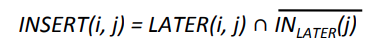
\includegraphics[width=0.6\textwidth]{p96.png}
         
         \label{fig:p96}
\end{figure}


There	are	different	insertion	points,	depending	on	the	
structure	of	the	CFG,	if	x $\in$ INSERT(i,	j):	

\begin{figure}[H]
    \centering
     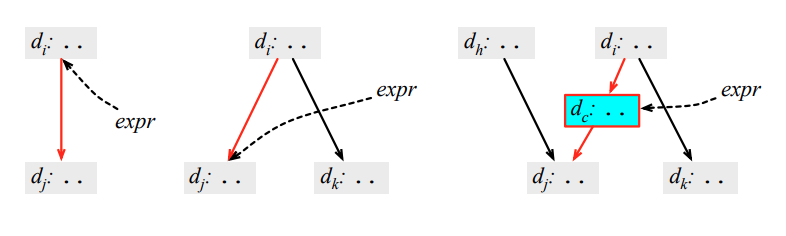
\includegraphics[width=0.6\textwidth]{p97.png}
         \caption{	Different	inser9on	points}
         \label{fig:p97}
\end{figure}
\subsection{Modify CFG}

Rename all compuation of the expression.  

\begin{figure}[H]
    \centering
     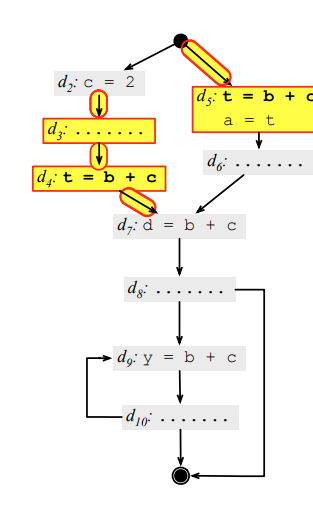
\includegraphics[width=0.4\textwidth]{p100.png}
         \caption{For \texttt{b+c}, the result of applyiny modifying CFG.}
         \label{fig:p100}
\end{figure}


\subsection{Which	Computations	to	Remove?	}
We	remove	computations	that	are	already	covered	by	
the	latest	points,	and	that	we	cannot	use	later	on.	

\begin{figure}[H]
    \centering
     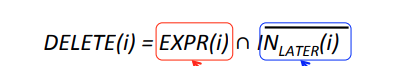
\includegraphics[width=0.6\textwidth]{p98.png}
         
         \label{fig:p98}
\end{figure}




For {\color{red} First} part, of	course,	the	expression	
must	be	used	in	the	block,	
otherwise	we	would	have	
nothing	to	delete. For {\color{blue} second} part, The	expression	may	not	be	a	
computation	that	is	necessary	
later	on.	


\begin{figure}[H]
    \centering
     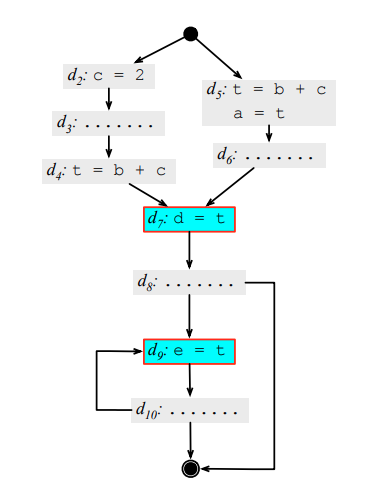
\includegraphics[width=0.4\textwidth]{p101.png}
         \caption{For \texttt{b+c}, the result of applyiny deleting redundancy \texttt{b+c}}
         \label{fig:p100}
\end{figure}



\subsection{A fully explained example}
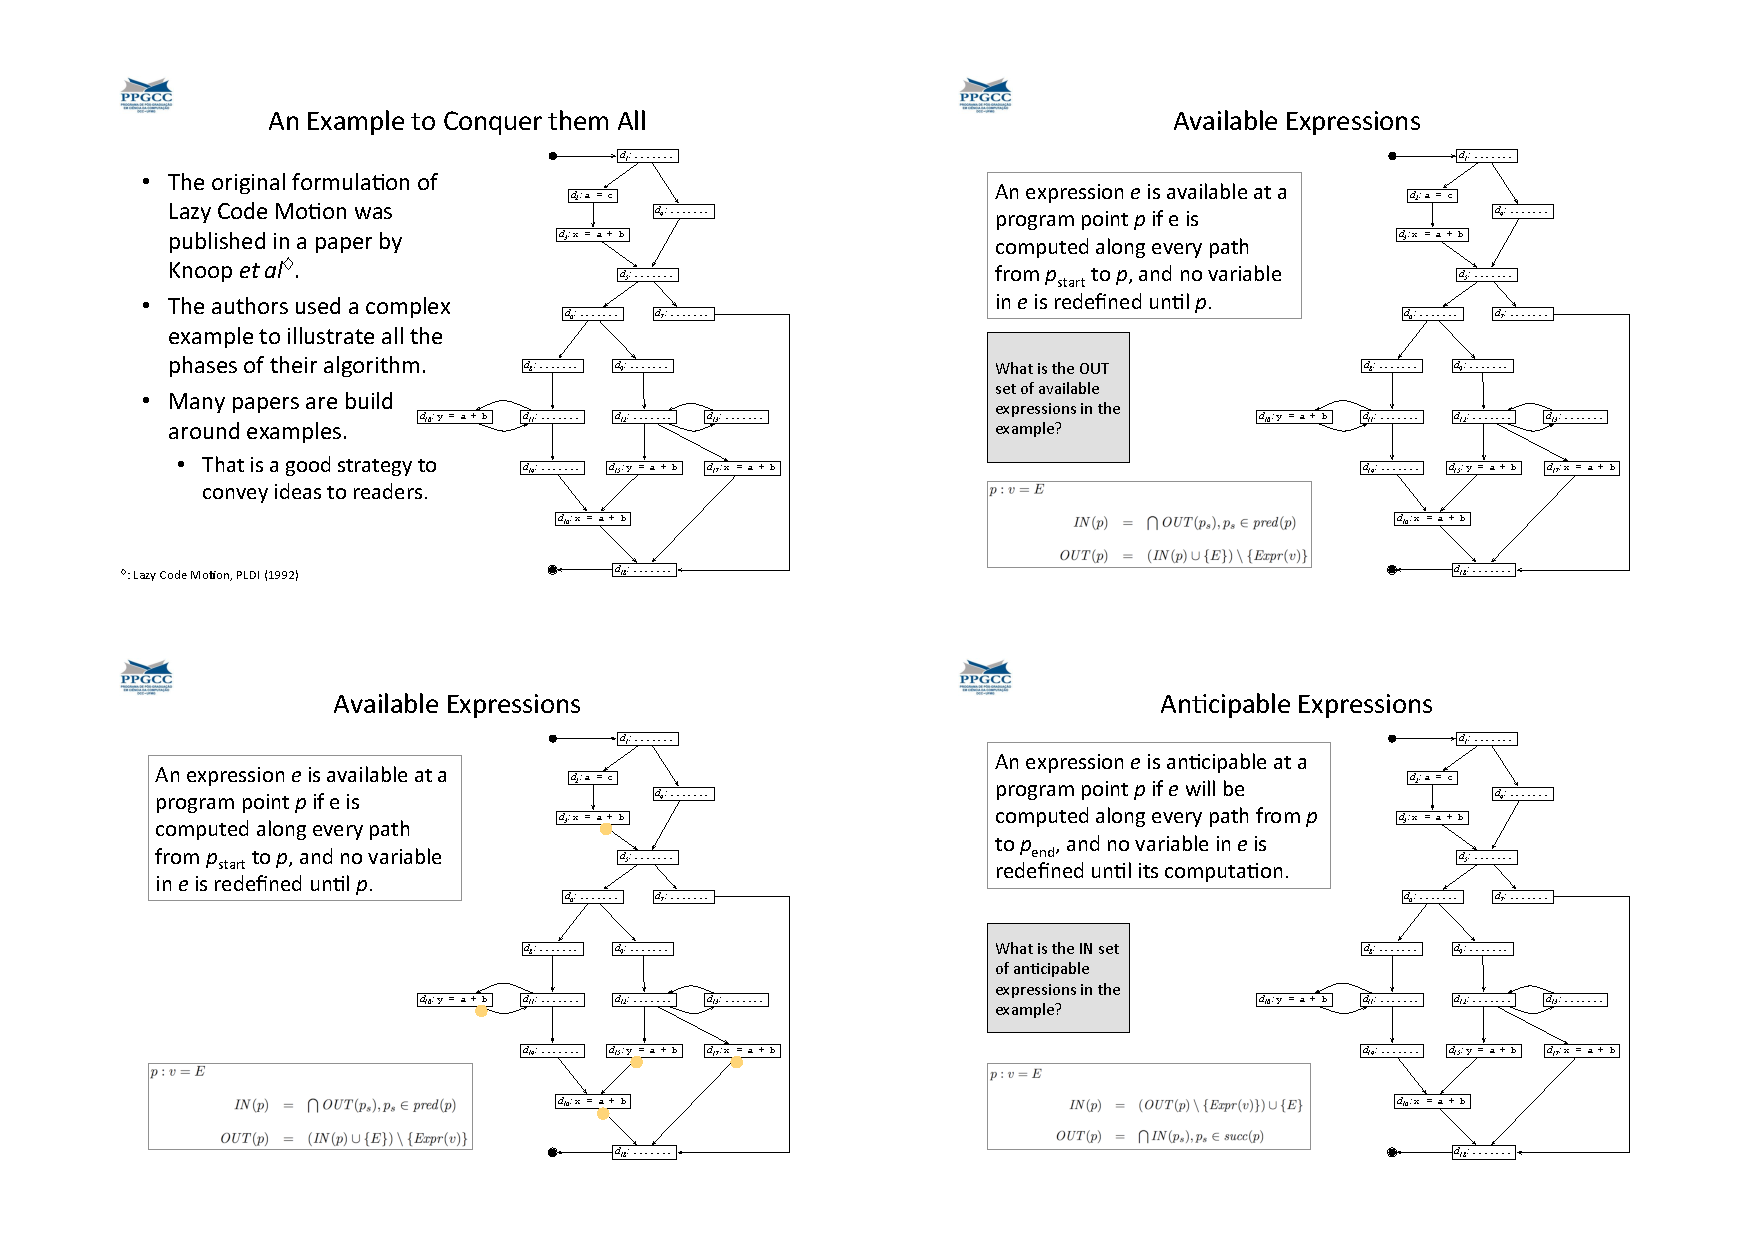
\includepdf[pages={1-}]{p99.pdf}


% We’ll start with an “enabling term.”

% \[
%     \mathrm{CONST}[i] = \mathrm{ANTIN}[i] \cap ( \mathrm{PAVIN}[i] \cup ( \neg \mathrm{KILL}[i] \cap \neg \mathrm{ANTLOC[i]}  ))
% \]


% This term say that we require the
% expression to be:

% \begin{itemize}
%     \item  Anticipated at the start of block i (somebody wants the expression) \\
%     {\large \textbf{and}} 
    
%         \item {\large \textbf{(2a)}}  The expression must be partially
%         available (to perhaps transform
%         into full availability)\\
%         {\large \textbf{or}} 
%         \item {\large \textbf{(2b)}} The block neither kills nor
%         computes the expression.
   
% \end{itemize}

% Next, we compute PPIn[i] and PPOut[i]
% .
% PP means “possible placement” of a computation at the start (PPIn[i]) or
% end (PPOut[i]) of a block. These values determine whether a
% computation of the expression would
% be “useful” at the start or end of a
% basic block.


% $$
% \text { PPOUT[i] }=\left\{\begin{array}{cl}
% 0 & i=\text { entry } \\
% \bigcap_{s \in \text { succ(i) }} \operatorname{PPIN}[\mathrm{s}] & \text { otherwise }
% \end{array}\right.
% $$

% We try to move computations "up" (nearer the start block). It makes sense to compute an
% expression at the end of a block if it
% makes sense to compute at the start
% of all the block’s successors.

% $$
% \operatorname{PPIN}[\mathrm{i}]=\left\{\begin{array}{cc}
% 0 & i=\text { exit } \\
% \text { ([ANTLOC[i] } \cup(\mathrm{PPOUT}[i]-\mathrm{KILL}[i])] & \\
% \bigcap_{p \in \text { preds(i) }}(\mathrm{PPOUT}[\mathrm{p}] \cup \mathrm{AVOUT}[\mathrm{p}]) & \text { otherwise } \\
% \cap \text { CONST[i]) }
% \end{array}\right.
% $$


% To determine if PPIni
%  is true, we first
% check the enabling term. It makes sense
% to consider a computation of the
% expression at the start of block i if the
% expression is anticipated (wanted) and
% partially available or if the expression is
% anticipated (wanted) and it is neither
% computed nor killed in the block.
% We then check that the expression is
% anticipated locally or that it is
% unchanged within the block and possibly
% positioned at the end of the block.

% Finally, we check that all the block’s
% predecessors either have the expression
% available at their ends or are willing to
% position a computation at their end.
% Note also, the bi-directional nature of
% this equation.